\newpage
\subsubsection{Calcul de la couleur de l'objet}

La couleur des objets est donnée par une valeur comprise entre 0 et 360 degrés. La valeur correspond à la teinte de l'objet. Comme montré sur le schéma ci-dessous une valeur à 180 degrés (donc au milieu) correspondrait à du cyan.

\begin{figure}[h]
    \centering
    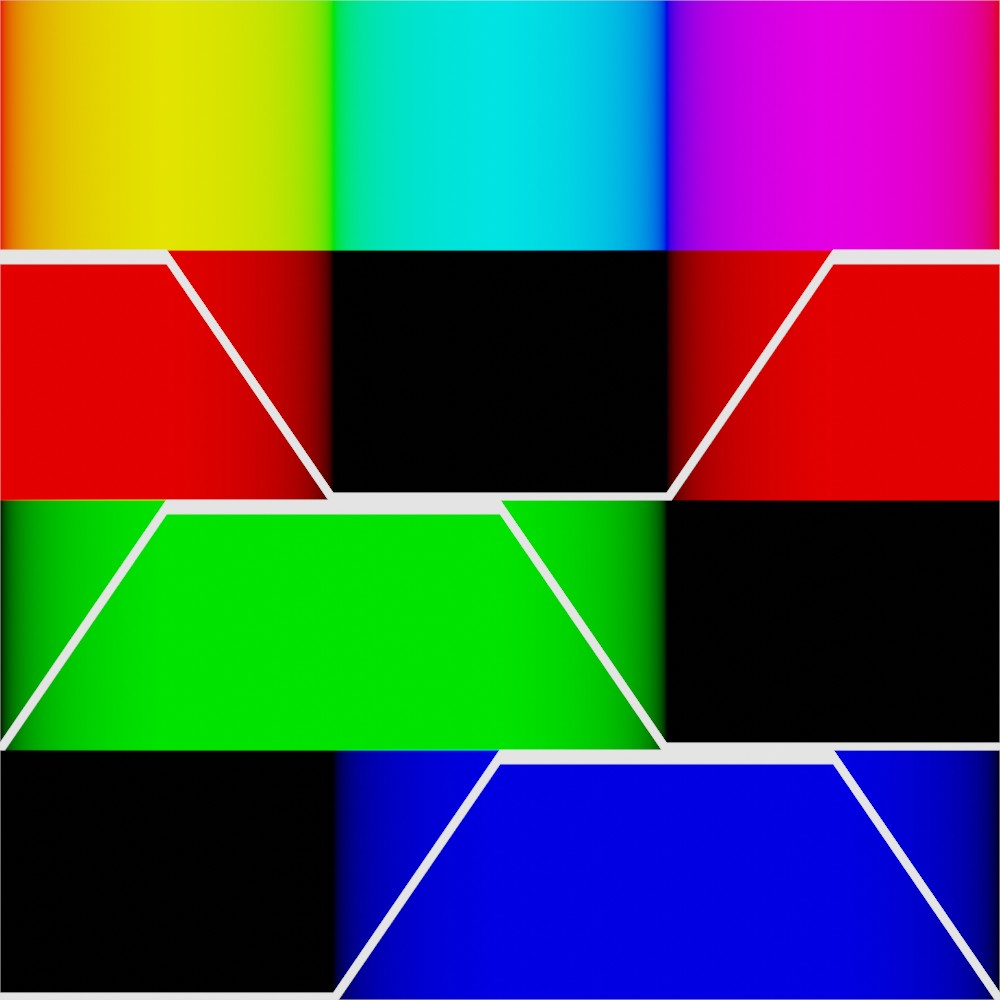
\includegraphics[width=8cm]{images/huetorgb.jpg}
    \caption{Décomposition de la couleur }
    \label{fig:huetorb}
\end{figure}

On remarque que l'on peut facilement calculer les valeurs de rouge de vert et de bleu (comprises entre 0 et 1) nécessaires à l'obtention de la coueleur souhaitée.\\
En effet, il suffit de découper la courbe tous les 60 degrés et on obtient des courbes constantes ou linaires.\\
Pour reprendre l'exemple du cyan, en se plaçant à 180 degré on remarque que le rouge vaut 0 et que le bleu et le vert valent 1.

\subsection{Calcul de la couleur à afficher}
\subsubsection{Calcul de normale}
Pour les calculs de couleurs, on va avoir besoin de la normale $\Vec{N}$ de la surface de l'objet "rencontré" par le rayon.
\begin{align*}
    \Vec{N}=normalize(\Vec{\nabla}SDF\_Scene(P))
\end{align*}
avec $normalize(\cdot )=\frac{\cdot }{\|\cdot \|}$\\
\\
\textbf{Remarque} : on utilise le fait que $SDF\_Scene$ est $\mathcal{C}^1(\mathbb{R}^3,\mathbb{R})$ sauf en certains points particuliers, comme par exemple à l'interieur d'un plan sans volume. Cependant, ces points critiques sont négligeables par rapport à la surface totale de l'objet. On évitera d'utiliser certaines figures, au profit d'autres ayant moins de discontinuités. Par exemple, on préférera utiliser un pavé très fin plutôt qu'un plan ayant deux dimensions.
\subsubsection{Calcul de l'éclairage}
On pose $LightPos \in \mathbb{R}^3$ la position d'une source de lumière et $LightColor$ sa couleur.
\\La contribution de cette source de lumière à l'éclairement d'un objet blanc de normale $\Vec{N}$ au point $\mathbf{P}$ est donnée par ce calcul : 
\begin{align*}
    Contribution=max(\left\langle \Vec{N},\ normalize(Lightpos-P) \right\rangle,\ 0) \times LightColor
\end{align*}
Il suffit de sommer la contribution de chaque source i de lumière :
\begin{align*}
    Couleur\_Pixel=\sum_{i=1}^{n} max(\left\langle \Vec{N},\ normalize(Lightpos_i-P) \right\rangle,\ 0) \times LightColor_i
\end{align*}
Avec n le nombre de sources de lumière
\textbf{Remarque} : Il n'est pas necessaire de gerer des problème de dépassement de couleur car le shader le fait lui-même.